\chapter{USP Kart}

O objetivo deste trabalho foi o desenvolvimento do jogo \textit{USP Kart}, um jogo de corrida estilo \textit{Kart} com temática da Universidade de São Paulo (USP). O jogo foi desenvolvido em C++ com OpenGL moderno e tem como principal característica a corrida com karts em um ambiente universitário, com personagens inspirados na mascote Fluffy.

Para isso foi escolhido uma lógica bidimensional, porém com gráficos tridimensionais, o que facilitou o desenvolvimento e permitiu que o jogo fosse lançado mais rapidamente. O jogo foi desenvolvido em duas máquinas, uma com Windows e outra com Linux, ou seja, tudo o que foi desenvolvido deve ser compatível com ambos os sistemas operacionais.

\section{Estilo artístico}

Como mencionado anteriormente, o jogo visa retratar uma corrida de karts em um ambiente universitário, dessa forma não utilizado modelos externos, mas a arte em geral foi desenvolvida pelos próprios desenvolvedores. A arte foi feita utilizando um programa de modelagem simples, o \textit{Blockbench} (\cite{prog:blockbench}), que permite a criação de modelos 3D simples e com baixa quantidade de polígonos.

Com exceção do mapa, todos os modelos foram feitos no \textit{Blockbench}, e a textura foi feita no \textit{GIMP} (\cite{prog:gimp}), um editor de imagens gratuito e de código aberto. A textura foi feita de forma simples, com cores sólidas e sem muitos detalhes, para manter a simplicidade e a leveza do jogo.

\pagebreak

\section{Personagens}

Todos os personagens seguem o mesmo modelo, e mesma textura, porém o jogo contém uma lógica de substituição de cores, permitindo que sua cor seja filtrada e substituída por outra, fazendo uma identificação única para cada personagem. Os personagens são inspirados na mascote Fluffy, e possuem uma textura simples, com cores sólidas e sem muitos detalhes.

\begin{figure}[H]
    \centering
    \begin{subfigure}[b]{1\textwidth}
        \centering
        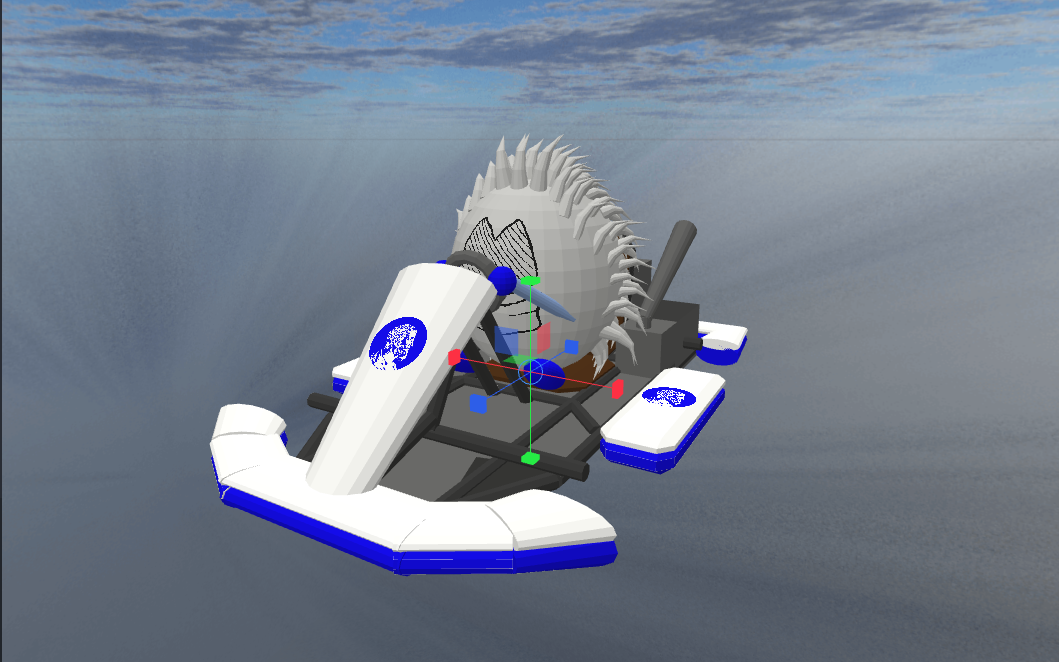
\includegraphics[width=0.8\textwidth]{figuras/Fluffy.png}
        \caption{Modelo do Fluffy no \textit{Blockbench}.}
        \label{fig:fluffy-blockbench}
    \end{subfigure}
    \begin{subfigure}[b]{1\textwidth}
        \centering
        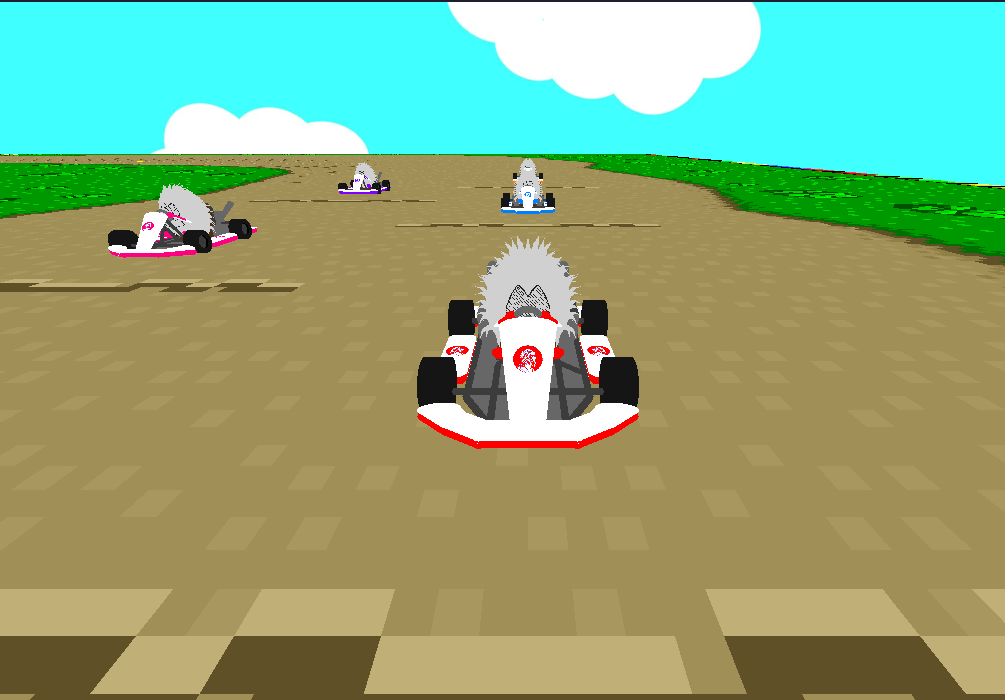
\includegraphics[width=0.8\textwidth]{figuras/USP Kart.png}
        \caption{Várias variantes do Fluffy com cores diferentes no USP Kart}
        \label{fig:fluffy-variantes}
    \end{subfigure}
    \caption{Fluffy no USP Kart.}
    \label{fig:fluffy}
\end{figure}

\section{Mapa}

O mapa é completamente em 2D, basicamente uma textura sólida com um caminho desenhado, ele não foi criado pelo desenvolvedor, mas teve de ser adaptado para o jogo. Esse mapa em específico se chama \textit{Donut Plains 1}, do \textit{Mario Kart} (\cite{marioKart}). O mapa é composto por um caminho principal e alguns atalhos, que podem ser utilizados para ganhar vantagem na corrida. Os atalhos são sutis e podem custar tempo se não forem utilizados corretamente.

\begin{figure}[H]
    \centering
    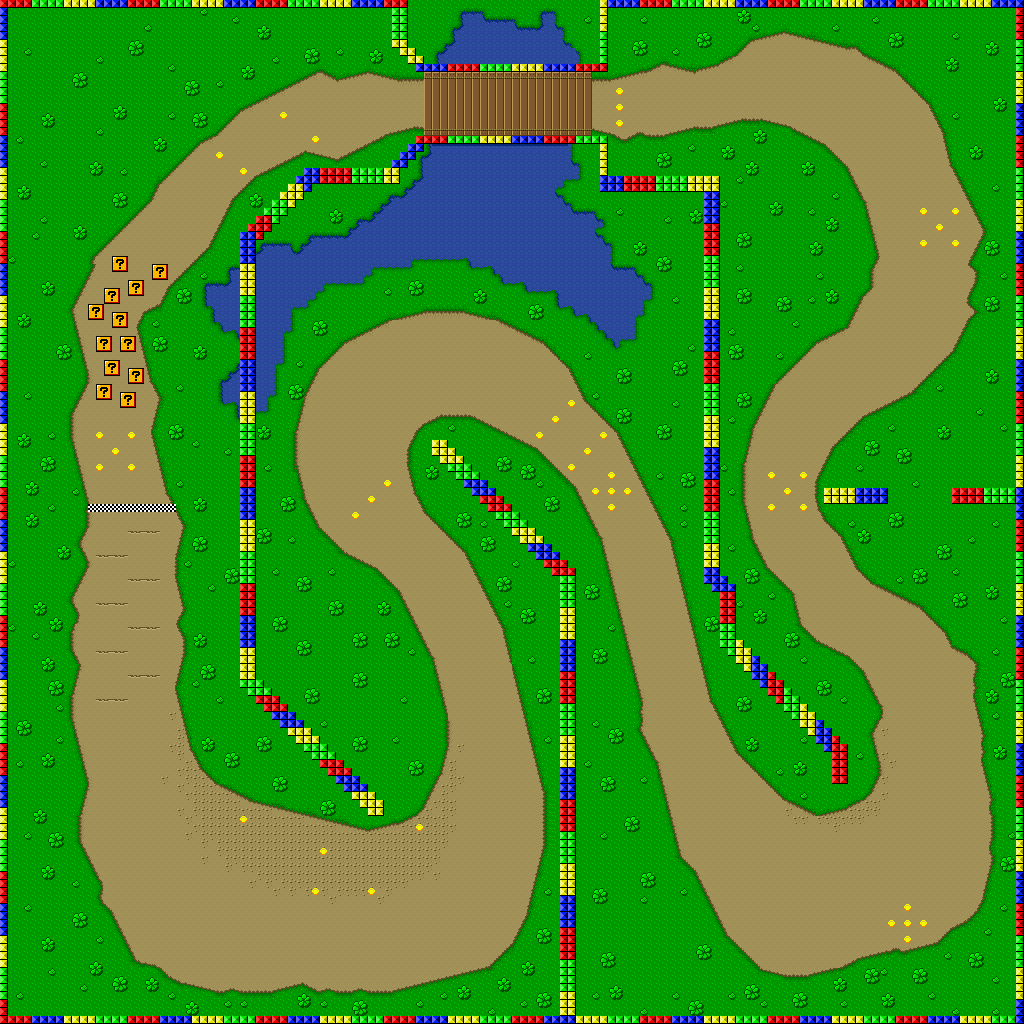
\includegraphics[width=0.8\textwidth]{figuras/Mapa.png}
    \caption{Mapa utilizado no USP Kart, Donut Plains 1. \cite{marioKart}}
    \label{fig:mapa}
\end{figure}


No mapa temos vários pontos de controle, apesar de invisíveis ao jogador, eles são utilizados para verificar se o jogador está no caminho correto, e caso não esteja, ele é incapaz de prosseguir. Os pontos de controle são extensos e poucos em quantidade, porém são o suficiente para garantir que o jogador esteja no caminho correto e não esteja trapaceando.

Também é válido notar que, com exceção do ponto de partida, todos os pontos de controle são o mais extensos o possível, fazendo com que o jogador possa passar por eles de qualquer direção, desde que esteja progredindo e se aproximando da linha de chegada. 

\section{Jogabilidade}

\textit{USP Kart} foi pensado para ser o mais responsivo o possível, utilizando do padrão de projeto \textit{State}, o personagem não realiza nenhuma ação além de mudar o seu estado, fazendo com que a transição de movimento seja muito mais suave e natural. O jogo também possui um sistema de colisão simples, mas eficaz, que permite que o personagem colida com objetos e outros personagens.

O jogador não possui nenhuma ação além de acelerar, frear e virar, o que simplifica a jogabilidade e permite que o jogador se concentre na corrida. Essas mesmas ações são utilizadas para todos os personagens, controlados pelo jogador ou não, fazendo com que as corridas sejam justas e equilibradas. O nome dessa técnica é \textit{rubber banding} (\cite{rubberBandAi}), que é uma técnica utilizada em jogos de corrida para manter a competição acirrada, mesmo que o jogador esteja muito à frente ou muito atrás dos outros.

Apesar disso, caso o jogador esteja muito atrás dos outros, os personagens controlados pela inteligência artificial (IA) diminuem a velocidade, permitindo que o jogador possa alcançá-los e ultrapassá-los. O contrário também acontece, caso o jogador esteja muito à frente, os personagens controlados pela IA aumentam a velocidade, permitindo que o jogador possa ser ultrapassado.

\section{Interface gráfica}

Apesar das bibliotecas utilizadas terem ajudado bastante no desenvolvimento do jogo, a interface gráfica se mostrou um grande desafio e é extremamente básica, consistindo de um texto no canto superior esquerdo da tela, que mostra a posição do jogador e a quantidade de quadros por segundo sendo desenhados, e um texto no canto superior direito da tela, que mostra a quantidade de voltas completadas.
